% 使用 ctexart 文档类，支持中文
\documentclass[12pt, a4paper]{ctexart}

% ========== 导言区：引入宏包并进行设置 ==========
\usepackage{geometry} % 用于设置页边距
\geometry{left=2.5cm, right=2.5cm, top=2.5cm, bottom=2.5cm}

\usepackage{graphicx} % 用于插入图片
\usepackage{float}    % 用于控制图片位置 [H]
\usepackage{caption}  % 用于自定义图表标题
\usepackage{amsmath, amssymb} % 用于数学公式
\usepackage{listings} % 用于插入代码
\usepackage{xcolor}   % 用于代码高亮颜色

% 设置代码块样式
\lstset{
    basicstyle=\ttfamily\small,
    keywordstyle=\color{blue},
    commentstyle=\color{green!60!black},
    stringstyle=\color{red},
    breaklines=true,
    numbers=left,
    numberstyle=\tiny,
    frame=single,
    tabsize=4
}

% 设置图表标题格式
\captionsetup[figure]{name=图, labelsep=period}
\captionsetup[table]{name=表, labelsep=period}

% ========== 正文开始 ==========

\begin{document}
% --- 标题与作者信息 ---
\begin{center}
    {\huge \textbf{Week2 }} \\[0.5cm]
    {\large 命令行环境；开发环境与工具；Debugging and Profiling} \\
    {\large 姓名：赵均临 \quad 学号：25020007178} \\
    {\large 日期：\today}
\end{center}
\vspace{0.5cm}
% --- 目录 ---
\tableofcontents
\newpage

github网址：https://github.com/coolicer17/Systemtools
% --- 第一章：课上实验题目 ---
\section{课上实验题目}
\subsection{实验5：控制一个可清理的后台任务}

\subsubsection{实现逻辑}
通过Shell \texttt{trap}捕获终止信号，结合作业控制实现后台任务的优雅退出，避免强制杀死进程导致资源泄漏。

\subsubsection{完整脚本 worker.sh}
\begin{lstlisting}
#!/usr/bin/env bash
trap 'echo "CLEAN_EXIT" >> cleanup.log; exit 0' TERM INT
n=0
while true; do echo "$n"; n=$((n+1)); sleep 1; done
\end{lstlisting}

\subsubsection{操作流程}
\begin{enumerate}
    \item 加权限启动：\lstinline|chmod +x worker.sh && ./worker.sh > stdout.log 2> stderr.log|
   \begin{figure}[H] % [H] 表示图片固定在此处
    \centering
    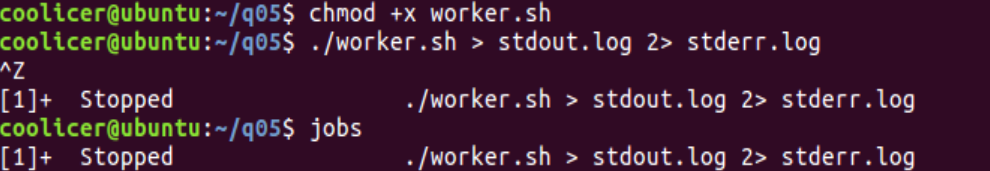
\includegraphics[width=0.9\textwidth]{data/5.2.png} % 请替换为你的图片文件名
    \label{fig:system}
\end{figure}
    \item 按Ctrl+Z挂起后执行 \lstinline|bg| 后台运行，\lstinline|jobs| 确认状态为Running
    \item 发信号终止：\lstinline|kill $(jobs -p)| （禁止用kill -9）
    \item \lstinline!SIGTERM!(15)可捕获允许清理，\lstinline!SIGKILL!(9)强制杀死不可拦截
\end{enumerate}
   \begin{figure}[H] % [H] 表示图片固定在此处
    \centering
    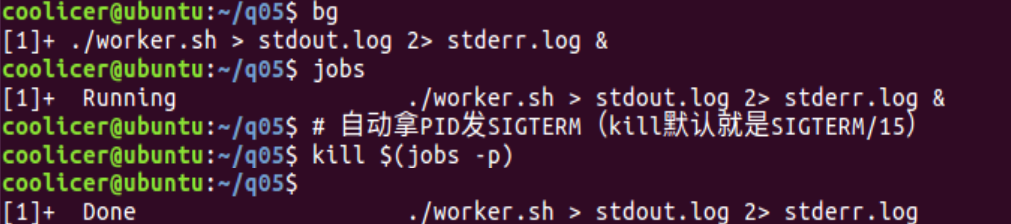
\includegraphics[width=0.9\textwidth]{data/5.3.png} % 请替换为你的图片文件名
    \label{fig:system}
\end{figure}
\subsubsection{核心知识点}
\begin{itemize}
    \item 信号区别：SIGTERM(15)可捕获允许清理，SIGKILL(9)强制杀死不可拦截
    \item 作业控制：\%N指代第N个作业，\texttt{bg/fg/Ctrl+Z}切换前后台运行状态
    \item trap命令：自定义信号处理动作，实现退出前的资源清理
\end{itemize}

\subsection{实验6：语义重构与本地开发反馈}
\subsubsection{实现逻辑}
利用现代代码编辑器的语言服务器协议（LSP）实现安全的语义重构，结合静态代码分析工具（ruff）和单元测试（pytest）保证代码质量与逻辑正确性。
\subsubsection{初始 Python 代码}
\subsection*{math\_utils.py}
\begin{lstlisting}
def total_price(price: float, count: int) -> float:
    return price * count
\end{lstlisting}

\subsection*{app.py}
\begin{lstlisting}
from math_utils import total_price

print(total_price(12.5, 4))
\end{lstlisting}

\subsection*{test\_math\_utils.py}
\begin{lstlisting}
from math_utils import total_price

def test_total_price():
    assert total_price(12.5, 4) == 50.0
\end{lstlisting}

\subsubsection{操作流程}
\begin{enumerate}
    \item \textbf{环境准备}：在编辑器中打开目录并确认 Python 语言服务器已激活。
    \item \textbf{语言特性演示}：使用 \texttt{F12} 跳转到定义，使用 \texttt{Shift+F12} 查找所有引用。
    \item \textbf{语义重构}：使用重命名符号（\texttt{F2}）将 \texttt{total\_price} 改为 \texttt{calculate\_total}，验证多文件引用同步更新。
    \item \textbf{静态检查与测试}：在 \texttt{app.py} 中故意加入 \texttt{import os}，运行 \texttt{ruff check . --fix} 自动剔除未使用导入，最后运行 \texttt{pytest} 确认测试通过。
\end{enumerate}

\subsubsection{核心知识点}
\begin{itemize}
    \item \textbf{LSP}：语言服务器协议提供代码跳转、引用查找和安全重命名能力。
    \item \textbf{Ruff}：极速的 Python 静态代码分析工具，可自动检测并修复未使用导入等问题。
    \begin{figure}[H] % [H] 表示图片固定在此处
    \centering
    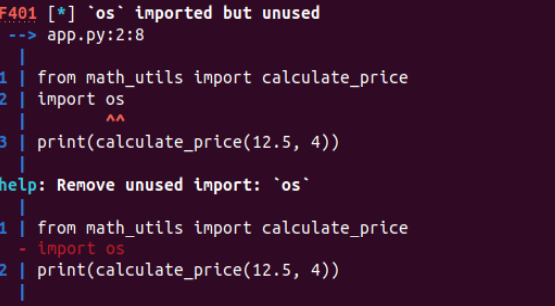
\includegraphics[width=0.7\textwidth]{data/6.1.png} % 请替换为你的图片文件名
    \label{fig:system}
    \end{figure}
    \item \textbf{Pytest}：自动化测试框架，用于回归验证重构后的代码逻辑。
\end{itemize}
    \begin{figure}[H] % [H] 表示图片固定在此处
    \centering
    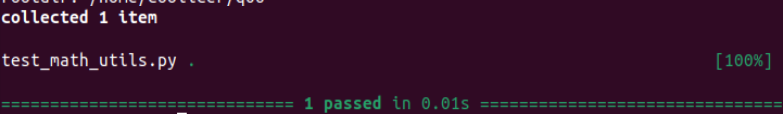
\includegraphics[width=0.8\textwidth]{data/6.2.png} % 请替换为你的图片文件名
    \label{fig:system}
\end{figure}

\subsection{实验7：用调试器定位归并排序缺陷}

\subsubsection{问题描述}
给定归并排序实现存在逻辑缺陷，要求不直接重写算法，通过调试定位问题并完成最小修复，同时补充单元测试验证正确性。

\subsubsection{缺陷代码分析}
原merge函数的else分支逻辑错误：当右数组当前元素更小时，错误地取左数组元素并移动右指针，直接导致右数组元素丢失，排序结果错乱。
\begin{lstlisting}[caption=带缺陷的merge片段]
while i < len(left) and j < len(right):
    if left[i] <= right[j]:
        result.append(left[i]); i += 1
    else:
        result.append(right[i]); j += 1      %-----wrong 
\end{lstlisting}

\subsubsection{调试过程}
1. 断点设置在merge函数入口，跟踪每次双指针比较过程
2. 观察到当`right[j] < left[i]`时，加入结果的是更大的left[i]，且右指针移动跳过更小元素
3. 确认循环结束后剩余拼接逻辑`result + left[i:] + right[j:]`本身正确，无需修改
\begin{figure}[H] % [H] 表示图片固定在此处
    \centering
    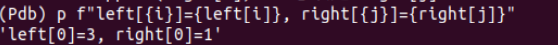
\includegraphics[width=0.9\textwidth]{data/7.3.png} % 请替换为你的图片文件名
    \label{fig:system}
\end{figure}
\subsubsection{修复后完整代码}
\begin{lstlisting}[caption=修复后的merge\_sort.py]
def merge(left, right):
    result = []
    i = j = 0
    while i < len(left) and j < len(right):
        if left[i] <= right[j]:
            result.append(left[i])
            i += 1
        else:
            result.append(right[j])
            j += 1
    return result + left[i:] + right[j:]

def merge_sort(a):
    if len(a) <= 1: return a
    m = len(a)//2
    return merge(merge_sort(a[:m]), merge_sort(a[m:]))
\end{lstlisting}

\subsubsection{测试结果}
运行pytest后两类用例全部通过：
- 给定随机输入排序结果与内置sorted完全一致
- 含大量重复元素的列表排序结果正确
- 空列表、单元素、逆序列表等边角场景均符合预期
\begin{figure}[H] % [H] 表示图片固定在此处
    \centering
    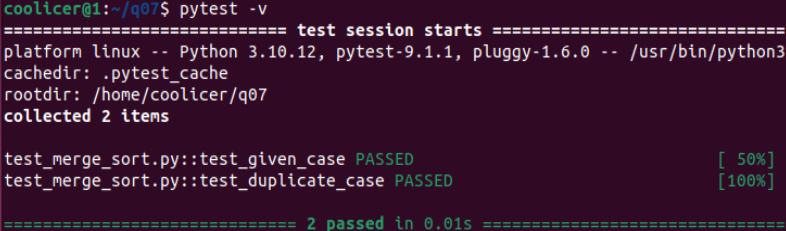
\includegraphics[width=0.9\textwidth]{data/7.2.png} % 请替换为你的图片文件名
    \label{fig:system}
\end{figure}
\subsubsection{核心知识点}
\begin{itemize}
    \item 双指针归并排序的核心逻辑：始终取两个数组头部的最小元素
    \item 调试器的断点、变量观察功能快速定位逻辑错误
    \item 单元测试用于回归验证重构/修复的正确性
\end{itemize}

\subsection{实验8：先测量，再优化慢速词频程序}

\subsubsection{原慢速代码}
\begin{lstlisting}
words = open("words.txt", encoding="utf-8").read().split()
unique = []
for word in words:
    if word not in unique:  # O(n) 
        unique.append(word)
print("count=", len(unique))
\end{lstlisting}

\subsubsection{操作流程}
\begin{enumerate}
    \item \textbf{生成数据}：运行 \texttt{generate\_words.py} 生成包含 30000 个随机词的 \texttt{words.txt}。
    \item \textbf{基线测量}：使用 \texttt{time python wordfreq.py} 运行 2 次，记录 \texttt{real} 时间并计算中位数[2](@ref)。
    \begin{figure}[H] % [H] 表示图片固定在此处
    \centering
    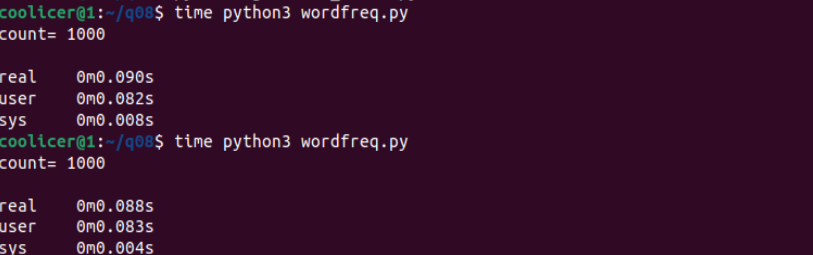
\includegraphics[width=0.9\textwidth]{data/8.1.png} % 请替换为你的图片文件名
    \label{fig:system}
\end{figure}
    \item \textbf{性能分析}：运行 \texttt{python -m cProfile -s cumulative wordfreq.py}，确认耗时集中在列表的 \texttt{\_\_contains\_\_} 操作上[1](@ref)。
    \begin{figure}[H] % [H] 表示图片固定在此处
    \centering
    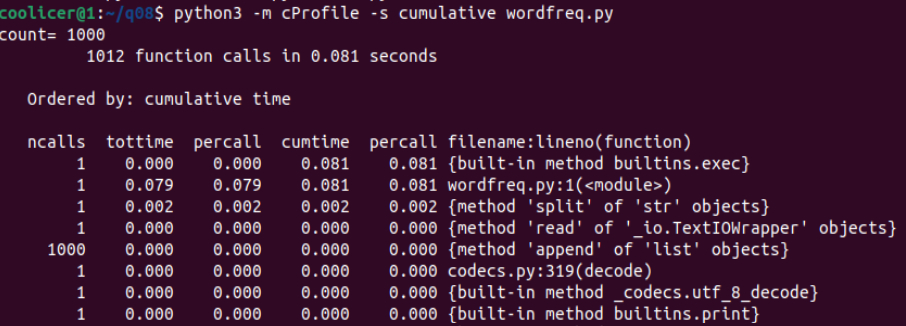
\includegraphics[width=0.9\textwidth]{data/8.2.png} % 请替换为你的图片文件名
    \label{fig:system}
\end{figure}
    \item \textbf{最小修复}：引入辅助 \texttt{set} 用于快速查重，保持原逻辑输出 \texttt{count} 不变。
    \item \textbf{优化后测量}：再次运行 \texttt{time} 命令 2 次，计算中位数与加速比。
    \begin{figure}[H] % [H] 表示图片固定在此处
    \centering
    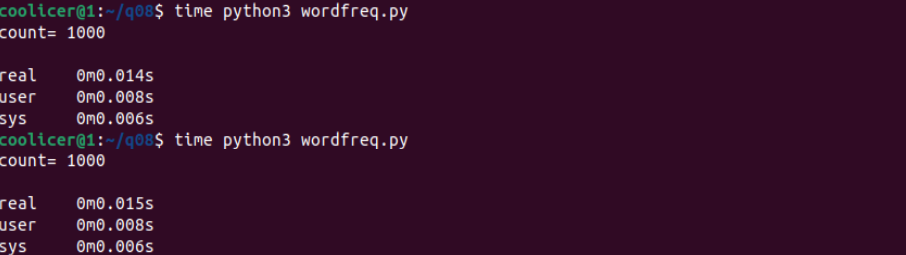
\includegraphics[width=0.9\textwidth]{data/8.3.png} % 请替换为你的图片文件名
    \label{fig:system}
\end{figure}
\end{enumerate}

\subsubsection{优化后代码}
\begin{lstlisting}
words = open("words.txt", encoding="utf-8").read().split()
seen = set()
unique = []
for word in words:
    if word not in seen:  # O(1) 
        seen.add(word)
        unique.append(word)
print("count=", len(unique))
\end{lstlisting}

\subsubsection{核心知识点}
\begin{itemize}
    \item \textbf{时间复杂度}：Python 列表的成员检测为 $O(n)$，集合（基于哈希表）为 $O(1)$。
    \item \textbf{Profiling}：\texttt{cProfile} 的 \texttt{-s cumulative} 参数可按累计耗时排序，快速定位热点函数[4](@ref)。
    \item \textbf{基准测试}：使用 \texttt{time} 命令多次运行取中位数，消除系统负载波动带来的误差。
\end{itemize}









% --- 第二章：练习 ---
\section{练习:命令行环境}

\subsection{参数与 Globs}
\subsubsection{-- 参数的作用}
\textbf{操作与指令：}
\begin{lstlisting}[language=Bash]
touch -- -myfile
ls -l -- -myfile
rm -- -myfile
\end{lstlisting}
\textbf{原理解释：} \texttt{--} 告诉程序停止解析后面的选项（flag）。如果不加 \texttt{--}，\texttt{touch -myfile} 会被解析为传递了 \texttt{-m}、\texttt{-y} 等选项参数，从而报错。
    \begin{figure}[H] % [H] 表示图片固定在此处
    \centering
    
\includegraphics[width=0.9\textwidth]{data/10.1.png} % 请替换为你的图片文件名
    \label{fig:system}
\end{figure}
\subsection{ls 命令组合参数}
\textbf{操作与指令：}
\begin{lstlisting}[language=Bash]
ls -lah --color=auto
\end{lstlisting}
\textbf{原理解释：} \texttt{-a} 显示隐藏文件，\texttt{-l} 列表格式，\texttt{-h} 易读大小，\texttt{-t} 按修改时间排序，\texttt{--color=auto} 输出颜色。
    \begin{figure}[H] % [H] 表示图片固定在此处
    \centering
    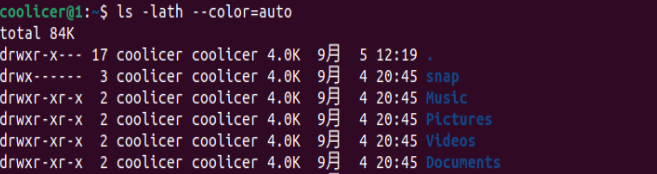
\includegraphics[width=0.9\textwidth]{data/10.1.2.png} % 请替换为你的图片文件名
    \label{fig:system}
\end{figure}
\subsection{环境变量与返回码}
\subsubsection{marco 与 polo 函数}
\textbf{操作与指令：} 创建 \texttt{marco.sh}：
\begin{lstlisting}[language=Bash]
#!/bin/bash
marco() { export MARCO_DIR=$(pwd); }
polo() { cd "$MARCO_DIR" || return; }
\end{lstlisting}
执行 \texttt{source marco.sh}。
    \begin{figure}[H] % [H] 表示图片固定在此处
    \centering
    
\includegraphics[width=0.8\textwidth]{data/10.2.png} % 请替换为你的图片文件名
    \label{fig:system}
\end{figure}
\subsection{循环调试脚本}
\textbf{操作与指令：}
\begin{lstlisting}[language=Bash]
#!/bin/bash
count=0
while true; do
    count=$((count+1))
    output=$(bash debug.sh 2>&1)
    if [ $? -ne 0 ]; then
        echo "Failed after $count runs"
        echo "$output"
        break
    fi
done
\end{lstlisting}
    \begin{figure}[H] % [H] 表示图片固定在此处
    \centering
    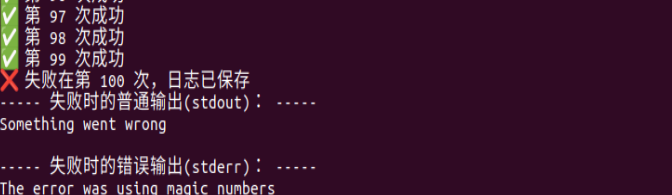
\includegraphics[width=0.8\textwidth]{data/10.3.2.png} % 请替换为你的图片文件名
    \label{fig:system}
\end{figure}
\subsection{信号与任务控制}
\subsubsection{后台任务处理}
\textbf{操作与指令：}
\begin{lstlisting}[language=Bash]
sleep 10000
#  Ctrl+Z 
bg
pkill -f "sleep 10000"
\end{lstlisting}
    \begin{figure}[H] % [H] 表示图片固定在此处
    \centering
    
\includegraphics[width=0.8\textwidth]{data/10.5.png} % 请替换为你的图片文件名
    \label{fig:system}
\end{figure}
\subsection{别名与点文件}
\subsubsection{纠错别名}
\textbf{操作与指令：}
\begin{lstlisting}[language=Bash]
alias dc='cd'
\end{lstlisting}

\subsection{远程机器 (SSH)}
\subsubsection{端口转发配置}
\textbf{操作与指令：} 编辑 \texttt{~/.ssh/config} 加入 \texttt{LocalForward 9999 localhost:8888}，服务端运行 \texttt{python -m http.server 8888}，本地访问 \texttt{http://localhost:9999}。
    \begin{figure}[H] % [H] 表示图片固定在此处
    \centering
    
\includegraphics[width=0.8\textwidth]{data/10.6.png} % 请替换为你的图片文件名
    \label{fig:system}
\end{figure}
    \begin{figure}[H] % [H] 表示图片固定在此处
    \centering
    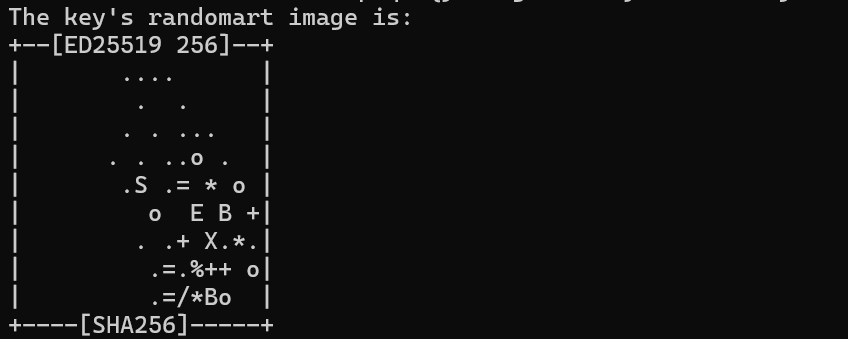
\includegraphics[width=0.7\textwidth]{data/10.6.2.png} % 请替换为你的图片文件名
    \label{fig:system}
\end{figure}
\section{练习： Debugging and Profiling}
\subsection{调试排序算法}
\subsubsection{归并排序 Bug 调试}
\textbf{操作与指令：}
\begin{lstlisting}[language=Bash]
gcc -g merge_sort.c -o merge_sort
gdb ./merge_sort
\end{lstlisting}
\textbf{原理解释：} 伪代码中切片语法需注意边界，实际实现中 \texttt{merge} 函数需正确处理数组剩余元素。
    \begin{figure}[H] % [H] 表示图片固定在此处
    \centering
    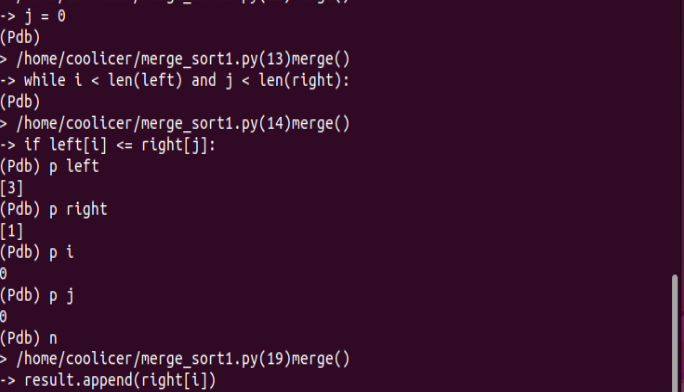
\includegraphics[width=0.8\textwidth]{data/10.7.png} % 请替换为你的图片文件名
    \label{fig:system}
\end{figure}
\subsection{反向调试}
\subsubsection{内存损坏排查}
\textbf{操作与指令：}
\begin{lstlisting}[language=Bash]
gcc -g corruption.c -o corruption
rr record ./corruption
rr replay
\end{lstlisting}
\textbf{原理解释：} \texttt{curve\_scores} 循环越界写入，覆盖了 \texttt{students[1].id}。

\subsection{AddressSanitizer}
\subsubsection{内存错误检测}
\textbf{操作与指令：}
\begin{lstlisting}[language=Bash]
gcc -fsanitize=address -g uaf.c -o uaf
./uaf
\end{lstlisting}
\textbf{原理解释：} Use-After-Free 错误。\texttt{free(greeting)} 后再次写入和读取。修复需删除 \texttt{free} 后的操作。
    \begin{figure}[H] % [H] 表示图片固定在此处
    \centering
    
\includegraphics[width=0.8\textwidth]{data/10.10.1.png} % 请替换为你的图片文件名
    \label{fig:system}
\end{figure}
    \begin{figure}[H] % [H] 表示图片固定在此处
    \centering
    
\includegraphics[width=0.7\textwidth]{data/10.10.2.png} % 请替换为你的图片文件名
    \label{fig:system}
\end{figure}


% --- 第四章：实验心得 ---
\section{实验心得}

在本周的实验中，我了解了什么是命令行以及如何去使用它，感受到了它强大的功能和便利的使用方式。并且学会了怎么对一个代码项目进行调试。
\par
通过实际操作，理解了信号捕获、作业控制、SSH 转发等命令行实用技巧
调试方面，体验了 gdb 断点、rr 反向调试与 AddressSanitizer 的高效定位能力。

\end{document}